\chapter{Background}
\label{ch:background}
For better understanding we introduce some topics before to analyze the problem. Each sections describe a general idea about it.

\section{Switched Systems}
Hybrid Systems are loosely defined as dynamical system whose state has two components, one of which evolves in a continuous set such as $\mathbb{R}$  while the other evolves in a discrete set such as $\mathbb{N}$ according to some transition logic based rule. The simplest model of a hybrid systems is given by: \citep{le2017improved}


\begin{figure}[!h]
    \begin{center}
        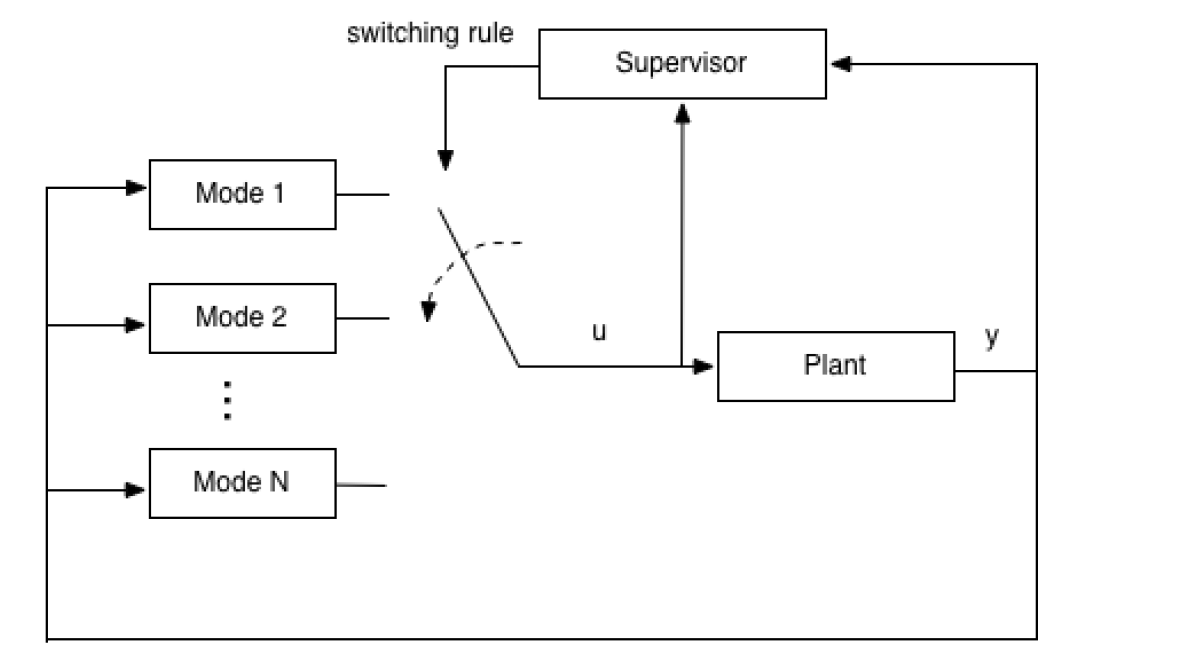
\includegraphics[width=\textwidth*4/5]{images/ss}
        \caption{Switched System Schematic}
    \end{center}
\end{figure}

\newpage
The figure above can be expressed as mathematical equation like this:
\begin{center}
    ${
    \dot x = f_{\sigma(t)}(x(t)), x \in \mathbb{R}^n,
    }$
    
    ${
    \sigma(t) = lim \phi(x(\tau),\sigma(\tau)), \sigma \in \mathbb{N},
    }$
\end{center}

\begin{figure}[!h]
    \begin{center}
        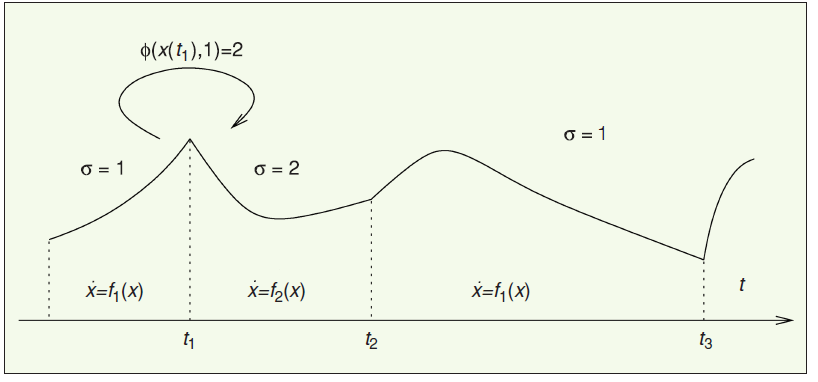
\includegraphics[width=\textwidth*4/5]{images/swiched}
        \caption{Trajectory of a hybrid system. The switching signal ${\sigma(t)}$ takes on integer values that change at discrete-time instances.\citep{liberzon2003switching}}
    \end{center}
\end{figure}




\section{Safety and Reachability}

In this part is presented a method based on correction by design of discrete linear switched system in the time. the method consist of given a objective region \emph{R} of state space, the method built a set \emph{S} and a control that guide any element from  \emph{S} a \emph{R}. This method works in an iterative way to back to reach the region \emph{R}. The method  can also be used for synthesize a stability control that is keep inside of R, whole states start in \emph{R}. \cite{le2016distributed}


 \textbf{Problem 1} \emph{((R,S) - Stability Problem)}. Given a switched system as shown in figure before, a set of recurrence ${\mathbb{R}^n}$ and a safe set \emph{S}
 
 ${\subset \mathbb{R}^n}$,find a control rule ${\sigma : \mathbb{R}^+ \rightarrow U}$ such that, for any initial condition ${x_0  \in  R_1}$ and any perturbation ${\varpi :\mathbb{R}^+\rightarrow U}$  the following holds:
 
 \begin{itemize}
    \item \emph{ Recurrence in \emph{R}:there are a monotonically strictly increasing sequence of (positive) integers
    ${k_t, t \in \mathbb{N}}$ such that for all ${ t \in \mathbb{R}^n, \phi(k_l\tau;t_0,x^0,\sigma,w) \in \mathbb{R} }$.}

    \item \emph{ Stability in \emph{S}: for all ${ t \in  \mathbb{R}^n, \phi(t;t_0,x^0,\sigma,w) \in S}$ .}
\end{itemize}
 
 
 \textbf{Problem 2} \emph{((${R_1,R_2,S}$) - Reachability proglem). Given a switched system of the form shown above, two sets  ${ R_1 \subset \mathbb{R}^n}$  and ${ R_2 \subset \mathbb{R}^n}$ and a safety set  ${S \subset  \mathbb{R}^n}$, find a control rule ${\sigma}$ : ${\mathbb{R}^+\rightarrow U}$ such that, for any initial condition ${x_0  \in  R_1}$ and any perturbation  ${\varpi : \mathbb{R}^+  \rightarrow U}$, the following holds:}
 
 \begin{itemize}
    \item  \emph{Reachability from ${R_1}$ to ${R_2}$: there exists an integer  ${k \in \mathbb{N} }$ such that we have ${ \phi( k_l\tau;t_0,x^0,\sigma,w) \in R_2 }$.}
    
    \item \emph{ Stability in S: for all ${ t \in \mathbb{R}^+, \phi(t;t_0,x^0,\sigma,w) \in S}$ .}
\end{itemize}
 
 \section{Switched Controller synthesis}

\textbf{Definition 1}\emph{(Sthocastic Hybrid Game)}. A stochastic hybrid game 
 
\textbf{Problem 3}\emph{(Control Synthesis Problem)}. Let us consider a sampled switched system. Given three sets R,S and B, with ${R \cup B \in S}$  and ${R \cap B = \varnothing }$ find a rule ${\sigma(.)}$ such that, for any ${x(0) \in R }$. 
 \begin{itemize}
    \item \emph{ ${\tau}$-stability: ${x(t)}$ return in R infinitely often, at some multiples of sampling time ${\tau}$}.
    \item \emph{ safety: ${x(t)}$ always stays in ${S/B}$.}
\end{itemize}




